\section{Examples: Concurrent Graph Mutation Conflicts}
\subsection{K-Clustering}
\begin{frame}{K-Clustering}
  \begin{itemize}
    \item Simplest unsupervised learning algorithm that solve the clustering problem.
    \item The process by objects are classified into number of groups so that they are as much dissimilar from one group to the other,
          and as much similar within each group.
    \item Grouping is done in the following fashion:
          \begin{itemize}
            \item Determine the centroid co-ordinate for each cluster
            \item Calculate the Euclidean distance from each object to the centroid of the cluster
            \item Group the object based on mimimum distance
          \end{itemize}
  \end{itemize}
\end{frame}

\begin{frame}{K-Clustering}
	Conflict in k-clustering algorithm
			\begin{figure}
			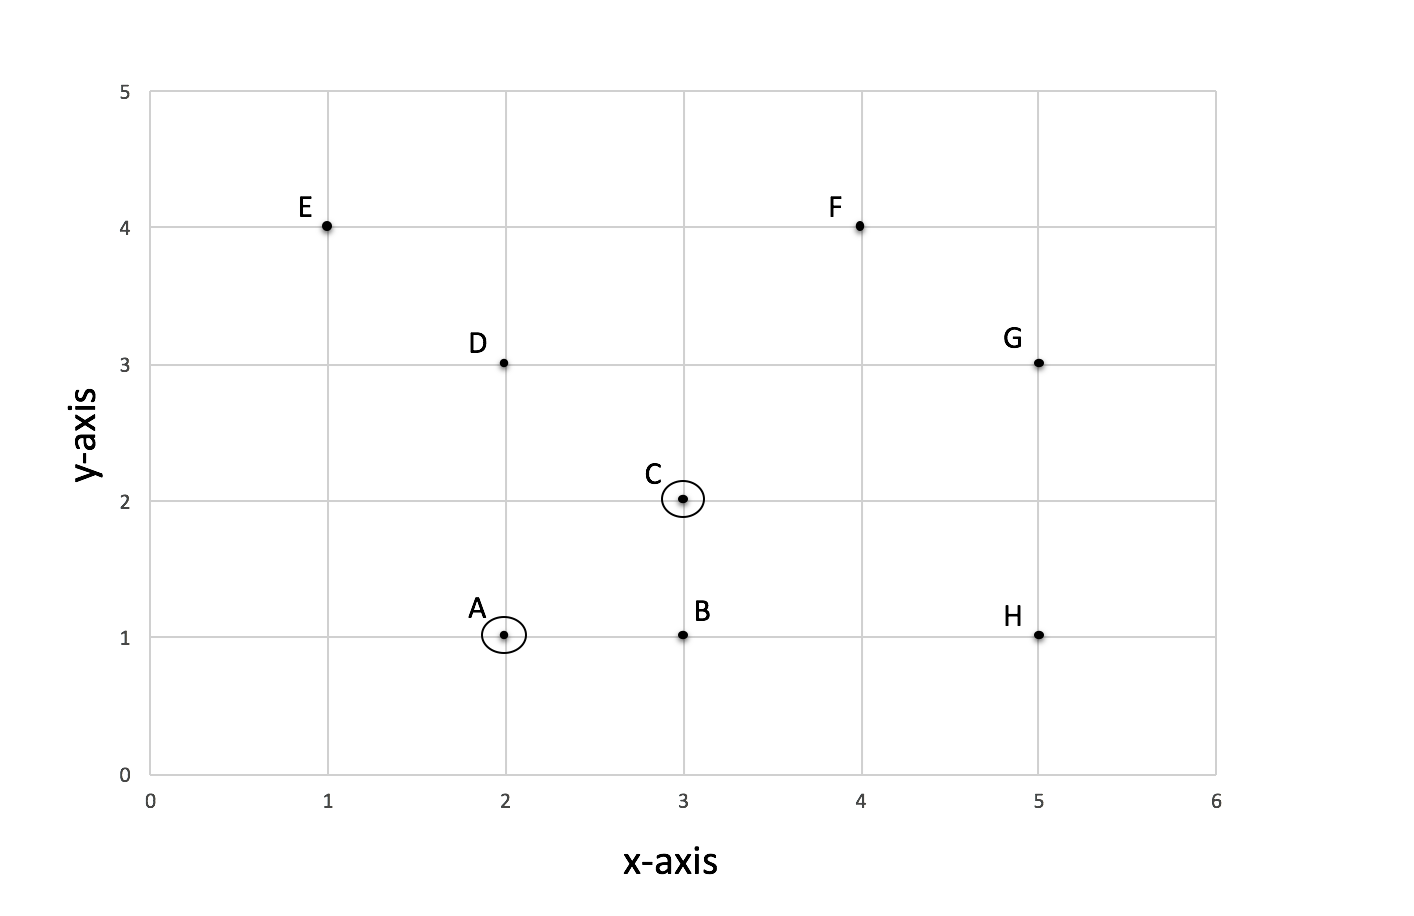
\includegraphics[width=0.8\linewidth]{figures/k-cluster.jpg}
			\caption{k-clustering algorithm}
			\end{figure}
\end{frame}

\begin{frame}{K-Clustering}
  Examples of Conflict in vertex related problems.\\
  1) K-Cluster Algorithm\\
  A=(2,1), B=(3,1), C=(3,2), D=(1,2),\\
  E=(1,0), F=(4,4), G=(5,3), H=(5,1)\\ where $B, D, E, F, G, H$ are objects\\
  $A$ and $C$ are two clusters.\\
\end{frame}

\begin{frame}{K-Clustering}
  Calculating Euclidean distance from each object to both of the clusters:\\
  $DA$=$\sqrt{{(1-2)}^2+{(2-1)}^2}=\sqrt{2}$,
  $DC$=$\sqrt{{(1-3)}^2+{(2-2)}^2}=2$\\
  $\therefore DA<DC$\\
  $BA$ = $\sqrt{{(3-2)}^2+{(1-1)}^2}=1$,
  $BC$ = $\sqrt{{(3-3)}^2+{(2-1)}^2}=1$\\
  $\therefore AB=BC$\\
  $AE$=$\sqrt{{(2-1)}^2+{(1-0)}^2}=\sqrt{2}$,
  $CE$=$\sqrt{{(3-1)}^2+{(2-0)}^2}=\sqrt{8}$\\
  $\therefore AE<CE$\\
\end{frame}

\begin{frame}{K-Clustering}
  $AF$=$\sqrt{{(4-2)}^2+{(4-1)}^2}=\sqrt{13}$,
  $CF$=$\sqrt{{(4-3)}^2+{(4-2)}^2}=\sqrt{5}$\\
  $\therefore CF<AF$\\
  $AG$=$\sqrt{{(5-2)}^2+{(3-1)}^2}=\sqrt{13}$,
  $CG$=$\sqrt{{(5-3)}^2+{(3-2)}^2}=\sqrt{5}$\\
  $\therefore CG<AG$\\
  $AH$=$\sqrt{{(5-2)}^2+{(1-1)}^2}=3$,
  $CH$=$\sqrt{{(5-3)}^2+{(1-2)}^2}=\sqrt{5}$\\
  $\therefore CH<AH$\\
\end{frame}
